% !TEX TS-program = pdflatex
% !TEX encoding = IsoLatin

%% Version 4x3 und 16x9  2.2 02.01.2014

% ==== wrapper class ==========================================================
\documentclass[% wrapper-class ETHpres option inspite of aspectratio for beamer-classe
    fourtothree=true, % true (default) -- 4:3-format, false -- 16:9-format
    DepLogo=true      % true -- use deplogo_13.pdf, false (default)
                      %         do not use deplogo_13.pdf for footer
    ]{include/ETHpres}

% ==== misc: you may use or not ===============================================
%\usepackage{graphicx}   % for including figures
%%\graphicspath{{pictures/}}
%\usepackage{tabularx}   % for special table environment (tabularx-table)
%\usepackage{booktabs}   % for table layout
%\usepackage{natbib}     % for bibliography with astron-style
%\bibliographystyle{astron}
%\usepackage{siunitx}    % to use for international units in the real world
%\usepackage[
%    colorlinks=true, linkcolor=white, urlcolor=white, % this is special for this presentation here to get the toc in white
%    hypertexnames=false,% for correct links (duplicate-error solution)
%	setpagesize=false,  % necessary in order to not change text-/paperformat for the document
%	pdfborder={0 0 0},  % removes border around links
%	pdfpagemode=FullScreen,% open pdf in full screen mode
%    pdfstartview=Fit    % fit page to pdf viewer
%]{hyperref}% all links stay black and are thus invisible

% ==== language ================================================================
\usepackage[latin1]{inputenc}
%\usepackage[utf8]{inputenc}
% English
\usepackage[english]{babel}
\AtBeginDocument{\renewcaptionname{english}{\contentsname}{\large Outline}}% toc-name
%% Deutsch
%\usepackage[ngerman]{babel}
%\AtBeginDocument{\renewcaptionname{ngerman}{\contentsname}{\large �bersicht}}% toc-name

% ==== choose the basic color for your presentation ===========================
% colorbar-color
\colorlet{firstcolor}{white} % see pages 2  and 3 of this sample presentation
% bachground color titlepage
\colorlet{secondcolor}{white} % see pages 2  and 3 of this sample presentation

\usepackage{amsmath}
\usepackage{algorithm}
\usepackage[noend]{algpseudocode}

% === fill in first information for the presentation ==========================
\newcommand*{\ETHtitle}{Creating wallpapers using mobile phone photos}
\newcommand*{\ETHauthor}{Seonwook Park}
\newcommand*{\ETHdate}{26.6.2015}
\begin{document}
% =========== begin of titlepage ============
\ETHtitelbild\textcolor{black}{\large\textbf{\ETHtitle}}
\newline
%%
% ==== start here with the text on the titlepage
%%
\textcolor{black}{\tiny{A semester project by Seonwook Park \\[-1.2mm]
Supervised by Michael Gygli and Dengxin Dai}}
\clearpage

\ETHminimal
\textbf{Outline\\}
\begin{itemize}
\item Introduction
\item Method
\begin{itemize}
	\item Suitability: Datasets, Training
	\item Cropping: Saliency, Features, Datasets
\end{itemize}
\item Results and Analysis
\item Summary
\item Further work
\end{itemize}
\clearpage

\ETHminimal
\textbf{Introduction\\}
\newline
\begin{minipage}{0.65\textwidth}
\begin{itemize}
	\item A mobile phone photo gallery contains a variety of images.
	\item Could use photos as wallpapers.
	\item Two challenges: Suitability and Cropping.
\end{itemize}
\end{minipage}
\begin{minipage}{0.4\textwidth}
	\begin{tikzpicture}[remember picture,overlay]
	  \node [xshift=-2.2cm,yshift=-4.1cm] at (current page.north east)
	    {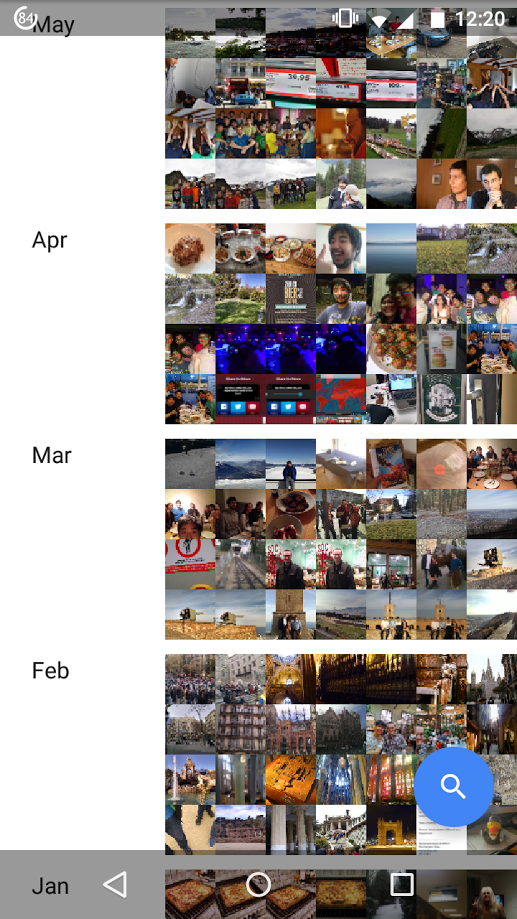
\includegraphics[width=3.2cm]{figures/mobile_gallery.png}};
	\end{tikzpicture}
\end{minipage}
\vspace{16mm}
\begin{itemize}
	\item Which image is suitable as a wallpaper?
	\item Which portion of a selected image should be visible?
\end{itemize}
\clearpage

\ETHminimal
\textbf{Method: Suitability - Datasets\\}
\newline
\begin{minipage}{0.65\textwidth}
\begin{itemize}
	\item Two datasets: Michael (275 images) and Wookie (266 images)
	\item Includes:
	\begin{itemize}
		\item Natural scenes
		\item Cityscapes
		\item Short-term memory
		\item Quick photos for messaging
	\end{itemize}
\end{itemize}
\end{minipage}
\begin{minipage}{0.4\textwidth}
	\begin{tikzpicture}[remember picture,overlay]
	  \node [xshift=-2.2cm,yshift=-4.1cm] at (current page.north east)
	    {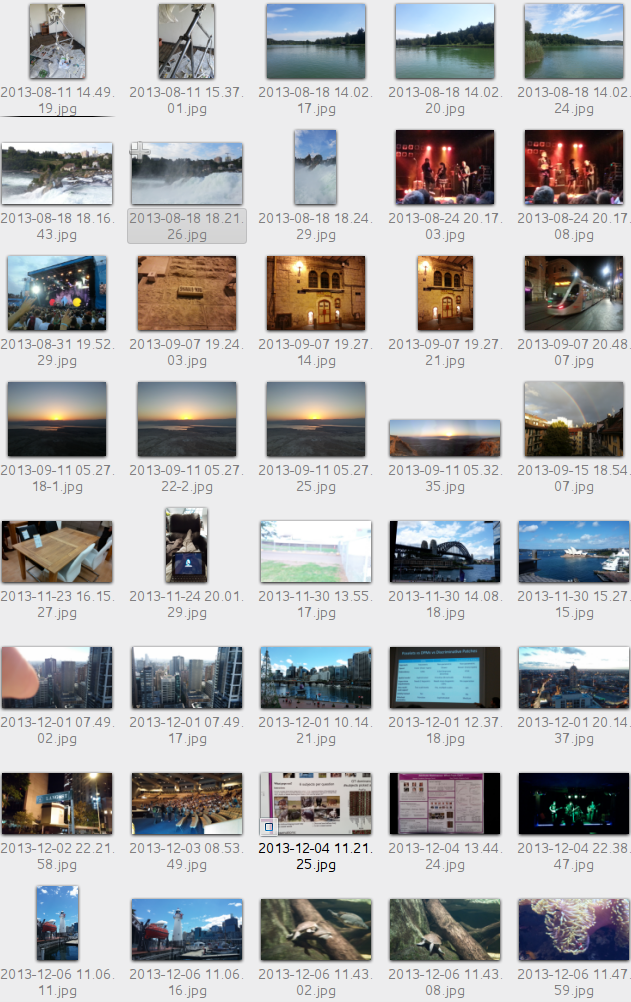
\includegraphics[width=3cm]{figures/michael_dataset.png}};
	\end{tikzpicture}
\end{minipage}
\clearpage

\ETHminimal
\textbf{Method: Suitability - Training\\}
\begin{itemize}
	\item Find objects in images to determine if suitable as a wallpaper.
	\item Done using Caffe, a deep learning library.
	\item Model used: BVLC Reference CaffeNet, 1000 object classes.
	\item Acquired feature vector used to train a SVM.
	\item SVM model trained on Wookie dataset. Michael dataset is used for evaluation.
\end{itemize}
\clearpage

\ETHminimal
\textbf{Method: Cropping - Saliency\\}
\begin{itemize}
	\item To crop an image, need to know what to keep.
	\item Distinctness compared to neighbouring regions.
	\item Aim to represent interesting regions in order to be able to
	      preserve information and yield well composed crops.
	\item Boolean Map based Saliency (BMS) by Zhang et al.
\end{itemize}
\clearpage

\ETHminimal
\textbf{Method: Cropping - Features\\}
\begin{figure}[h!]
\centering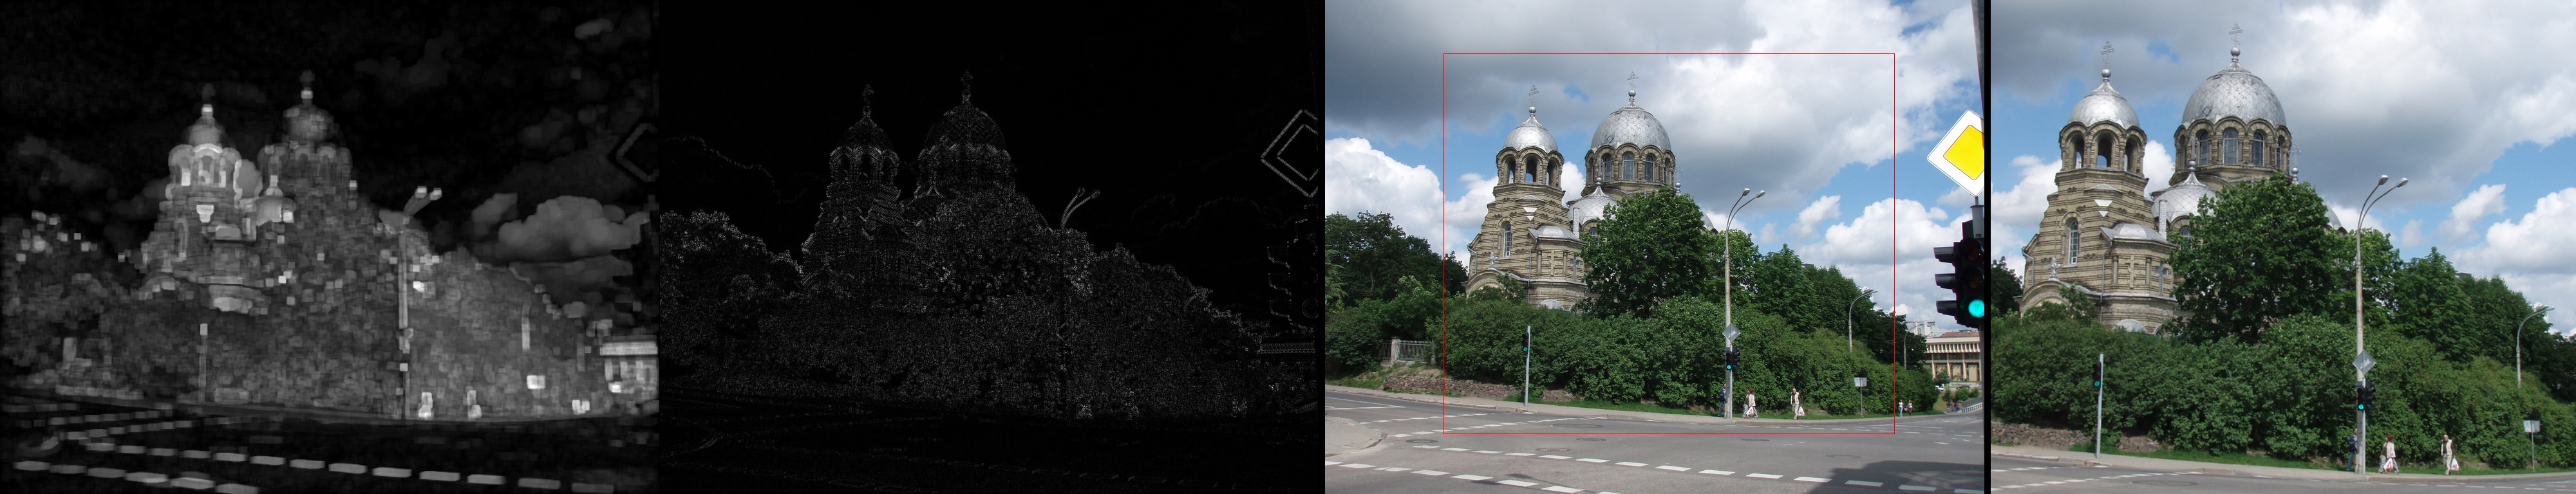
\includegraphics[width=11.5cm]{../figures/example_autocrop.jpg}
\end{figure}
\begin{enumerate}
	\item Saliency Composition
	\item Boundary Simplicity
	\item Content Preservation
\end{enumerate}
\clearpage

\ETHminimal
\textbf{Method: Cropping - Features}
\begin{itemize}
	\item 3-level spatial pyramid of saliency map
		\begin{itemize}
		\item $4\times4$ and $2\times2$ patches.
		\item $16 + 4 + 1 + 1 = 22$ features.
		\end{itemize}
	\item Boundary simplicity
		\begin{itemize}
		\item Gradient map using Sobel filter and \texttt{abs}.
		\item Mean value of 2-pixel wide strips used.
		\item $4$ features, $1$ per edge.
		\end{itemize}
	\item $26$ features in total. Used to train an SVM.
\end{itemize}
\clearpage

\ETHminimal
\textbf{Method: Cropping - Datasets}
\begin{itemize}
	\item Human crop dataset
		\begin{itemize}
		\item Collected from Amazon Mechanical Turks, Chen et al. (2014)
		\item 500 images, 10 crops per image.
		\item Used for evaluating model.
		\end{itemize}
	\item Reddit dataset
		\begin{itemize}
		\item Top 2000 images in the past year.
		\item Subreddits used: \tiny{CityPorn, EarthPorn, itookapicture, photocritique, WaterPorn, windowshots}\normalsize
		\item Used for training model.
		\end{itemize}
\end{itemize}
\clearpage

\makeatletter
\def\BState{\State\hskip-\ALG@thistlm}
\makeatother

\ETHminimal
\textbf{Method: Cropping - Final\\}
\begin{algorithm}
\scriptsize
\begin{algorithmic}[1]

\State $saliency \gets$ Saliency Map
\State $thresh \gets 0.7$
\State $n \gets 0$
    \Repeat
	\State Generate $5000$ crop candidates.
	\ForAll{crop}
		\State $cropped \gets saliency(crop)$
		\State $S\_content = sum(cropped) / sum(saliency)$
		\If{$S\_content < thresh$}
			\State Add crop to candidates
			\State $n = n + 1$
		\EndIf
	\EndFor
	\State $thresh = thresh * 0.95$
    \Until{n > 50}
\end{algorithmic}
\end{algorithm}
\clearpage

\ETHminimal
\textbf{Final pipeline}
\begin{figure}[h!]
\centering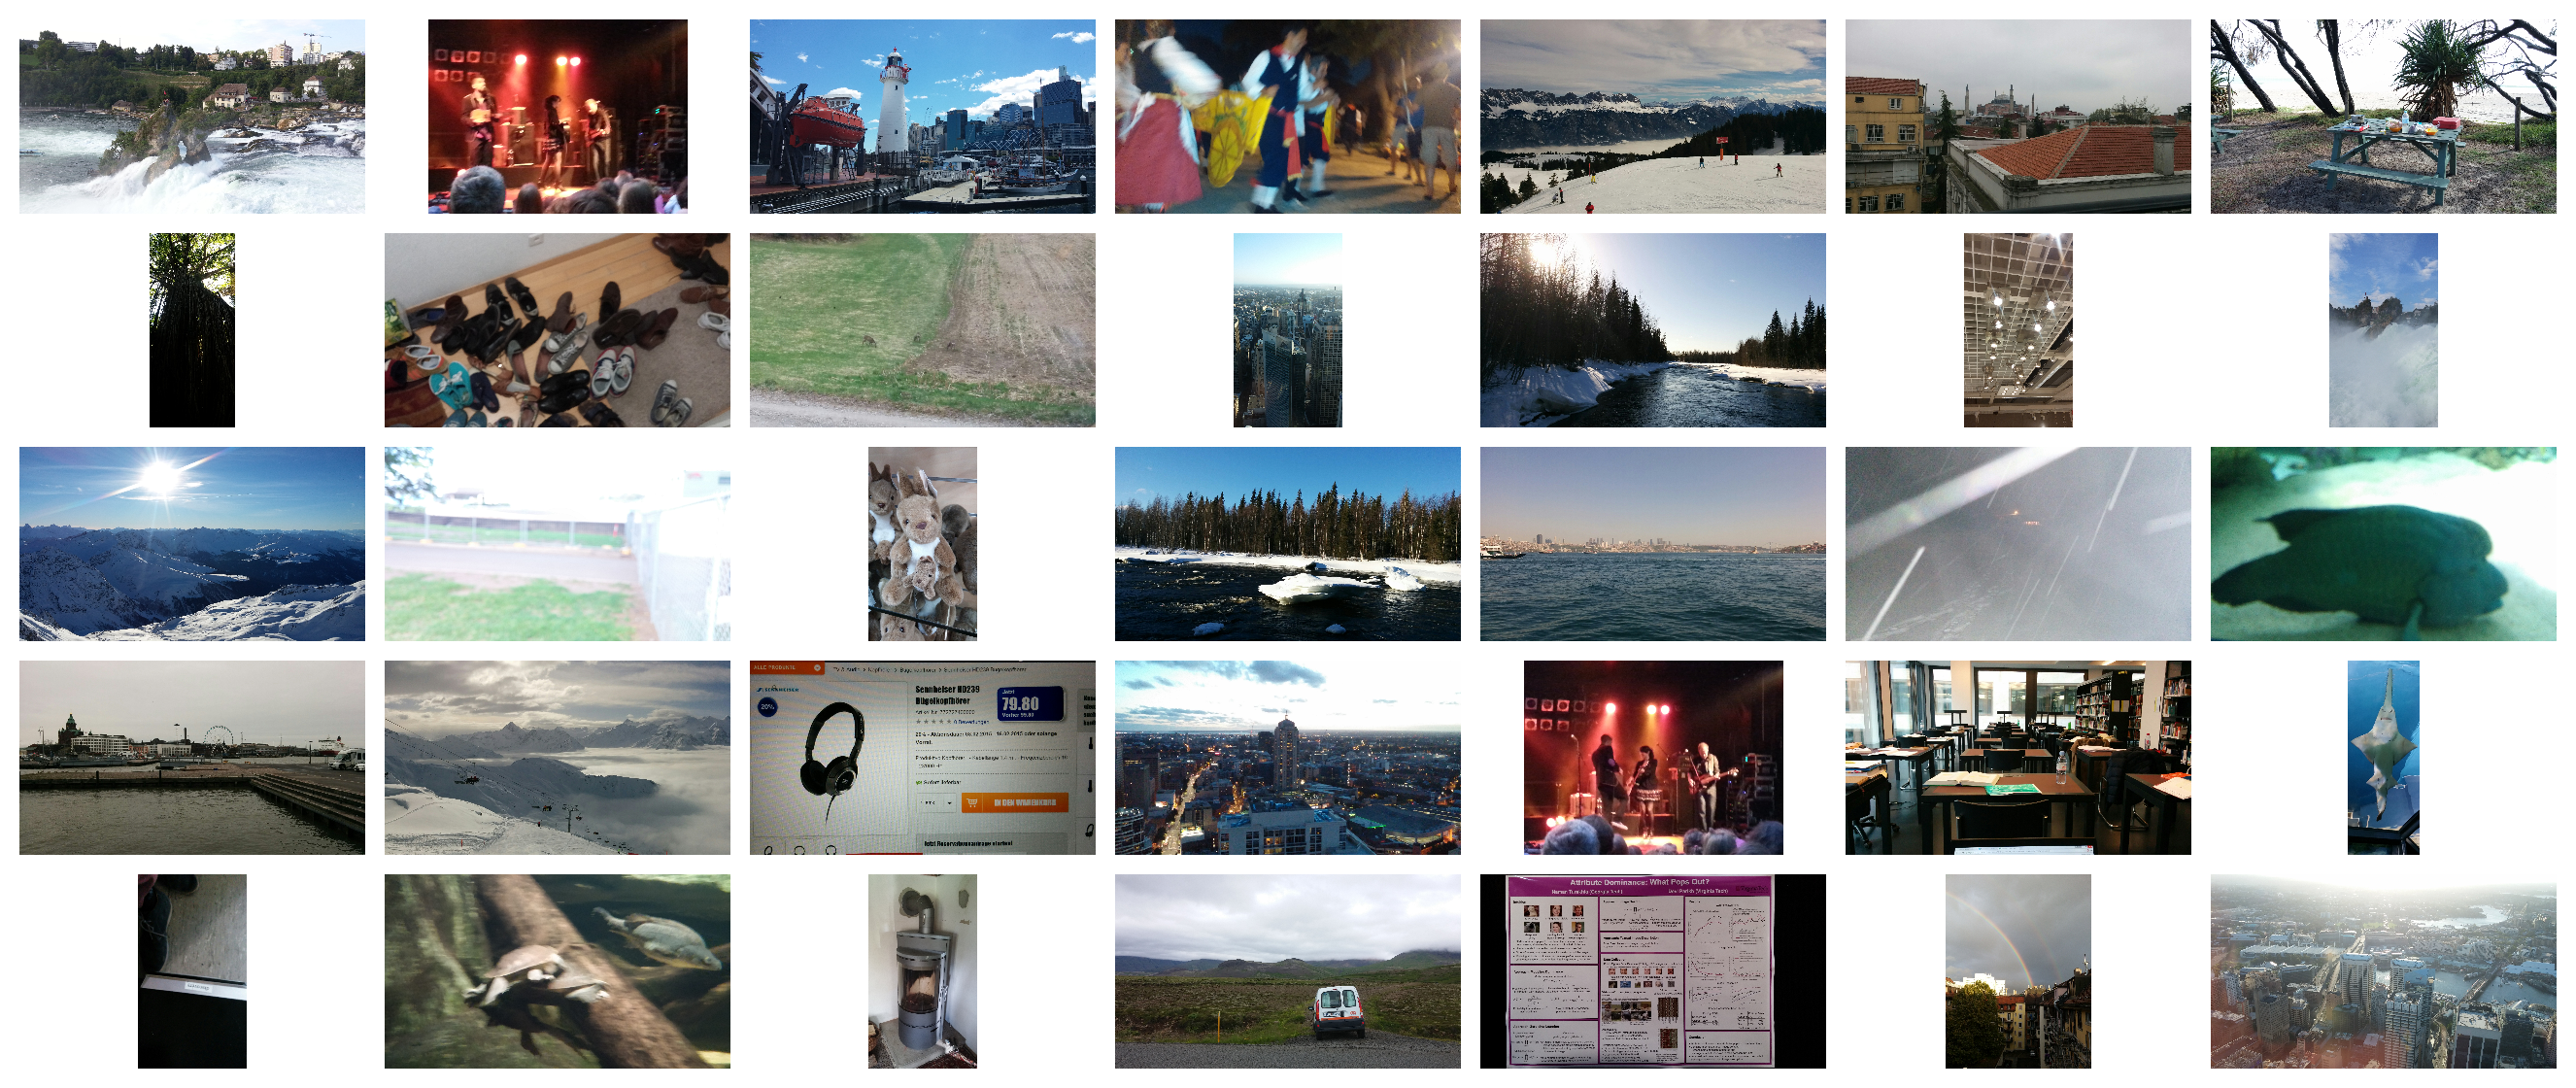
\includegraphics[width=11.5cm]{../figures/grid5x7_out1.png}
\end{figure}
\clearpage

\ETHminimal
\textbf{Final pipeline}
\begin{figure}[h!]
\centering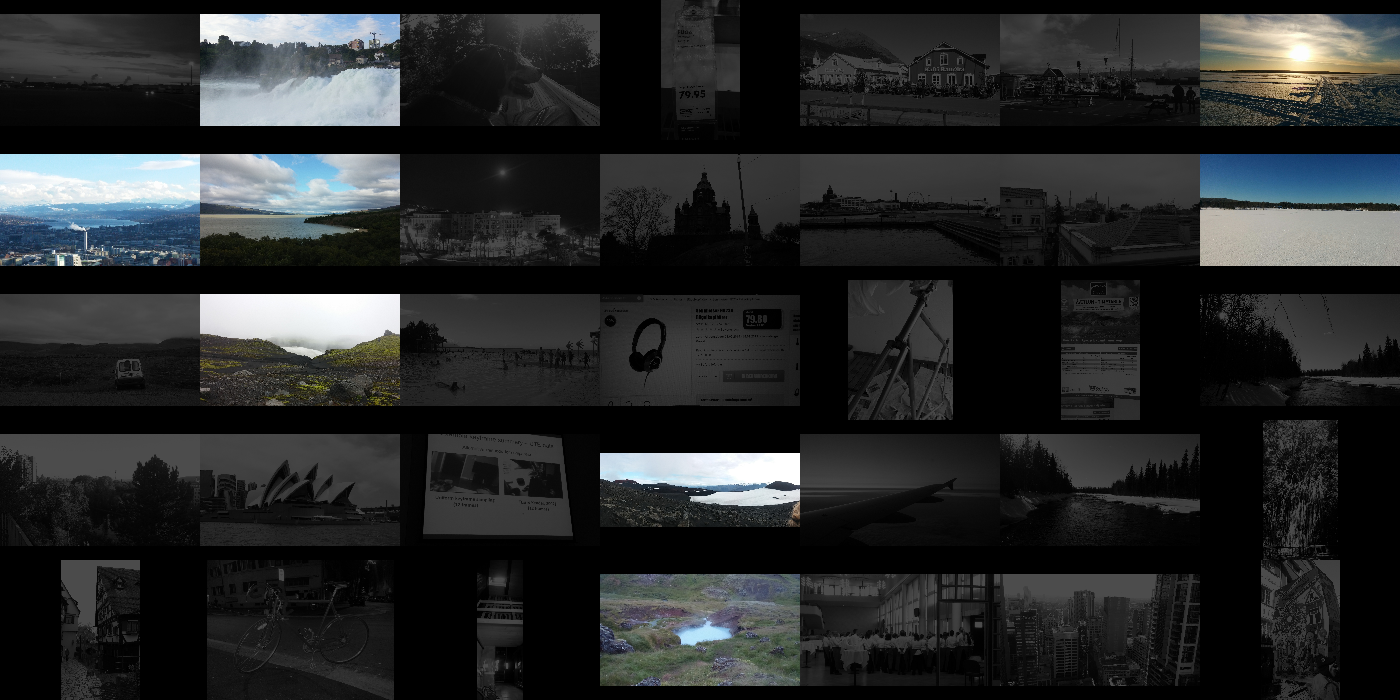
\includegraphics[width=11.5cm]{../figures/grid5x7_out2.png}
\end{figure}
\clearpage

\ETHminimal
\textbf{Final pipeline}
\begin{figure}[h!]
\centering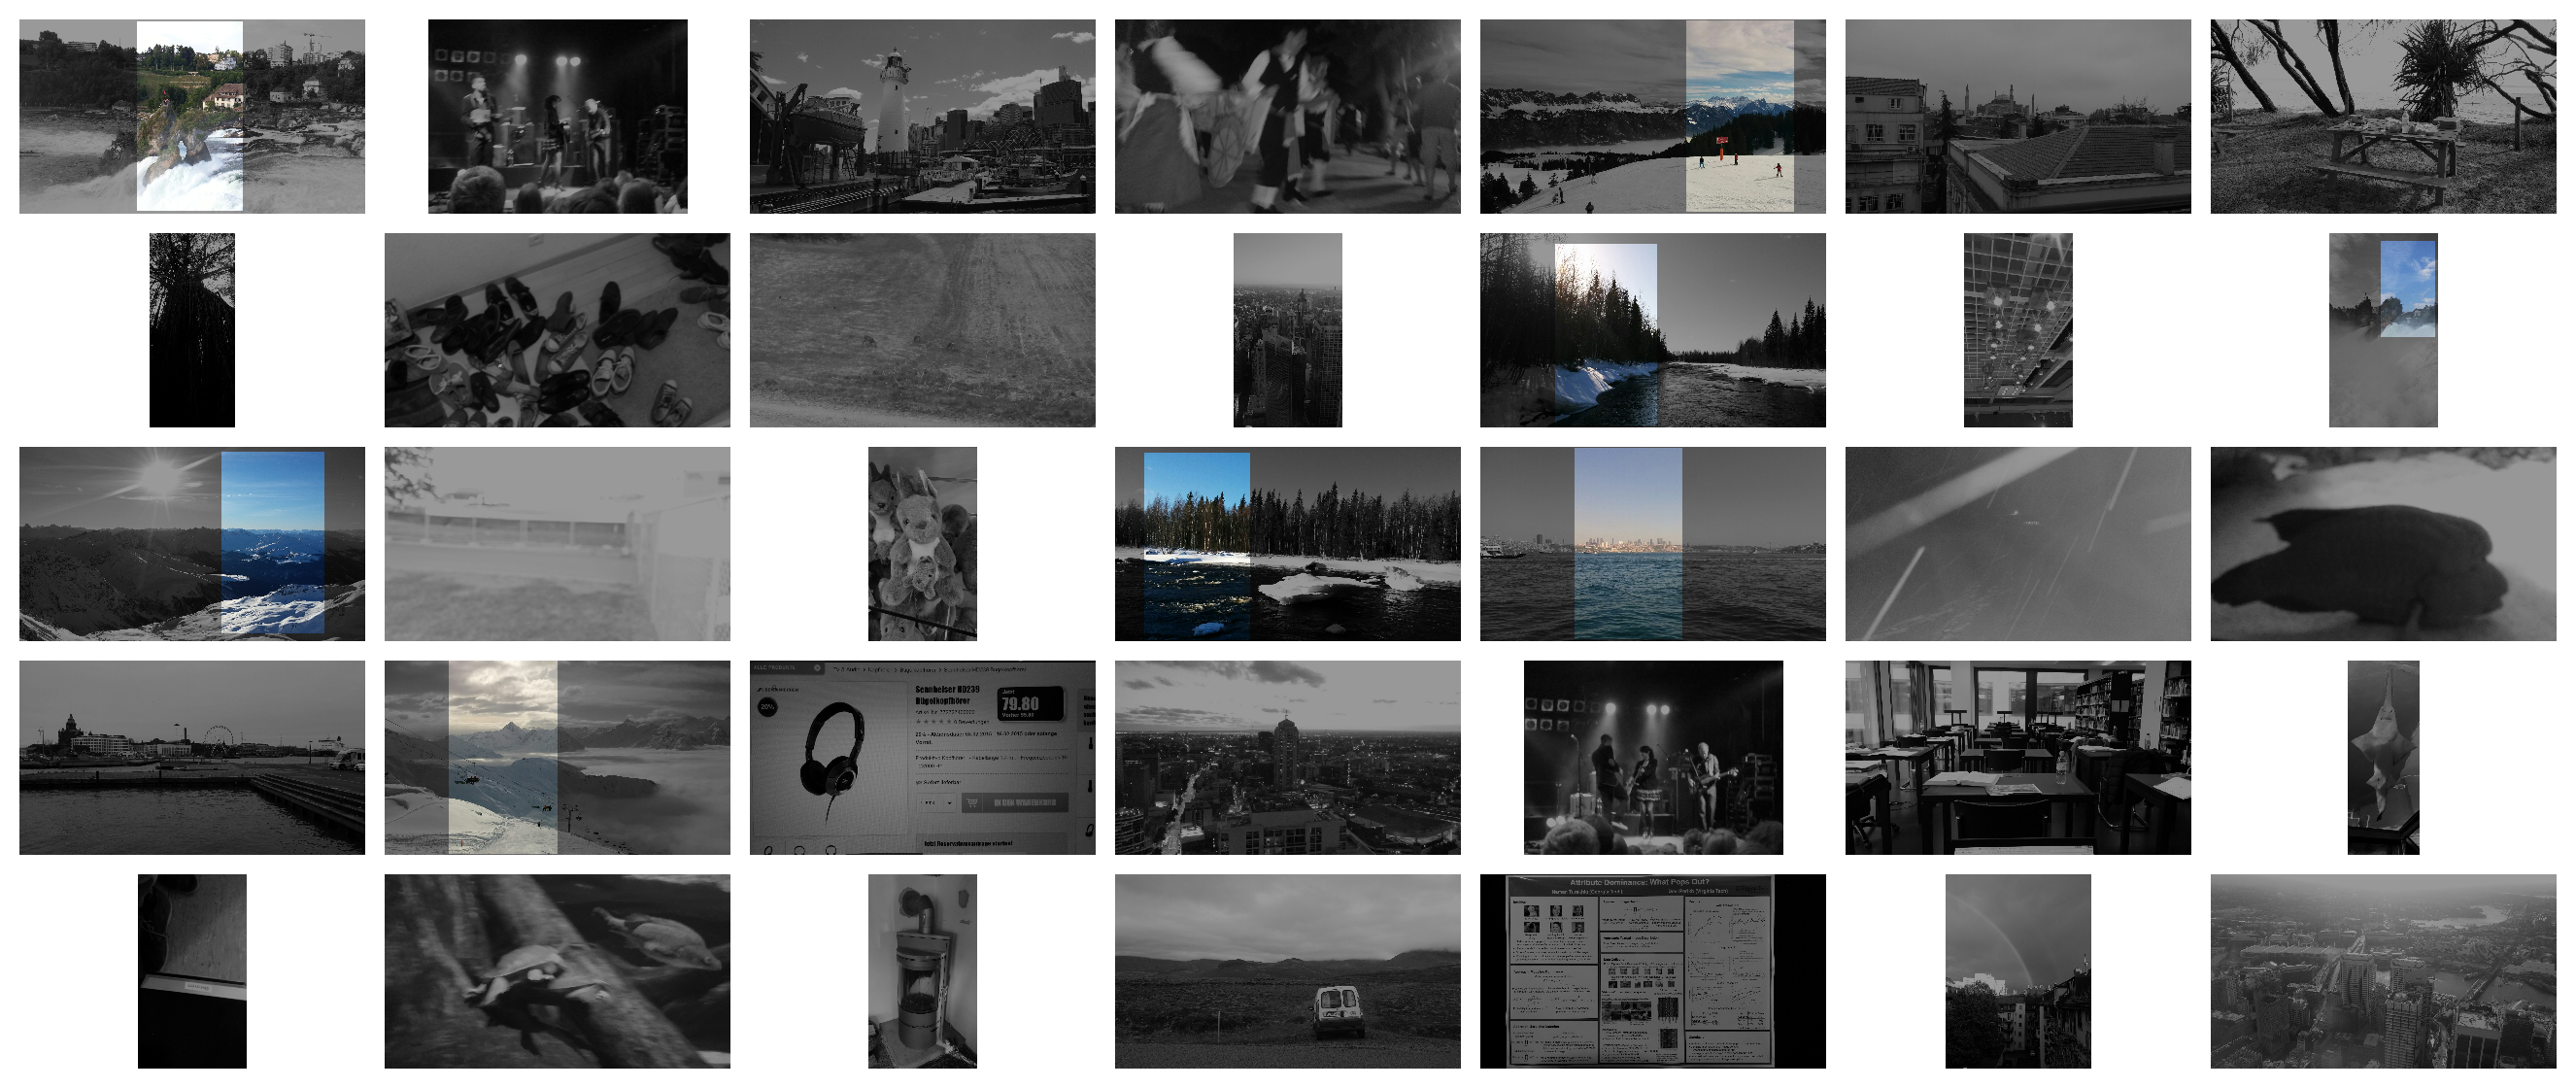
\includegraphics[width=11.5cm]{../figures/grid5x7_out3.png}
\end{figure}
\clearpage

\ETHminimal
\textbf{Analysis: Suitability\\}
\begin{itemize}
	\item Classifications gathered from four people.
	\item When considering images with consensus, misclassification error of
	      Michael set is $9.8\%$.
	\item $53$ out of $275$ images are considered suitable.
\end{itemize}
\clearpage

\ETHminimal
\textbf{Results: Cropping (Good)}
\begin{figure}[h!]
\centering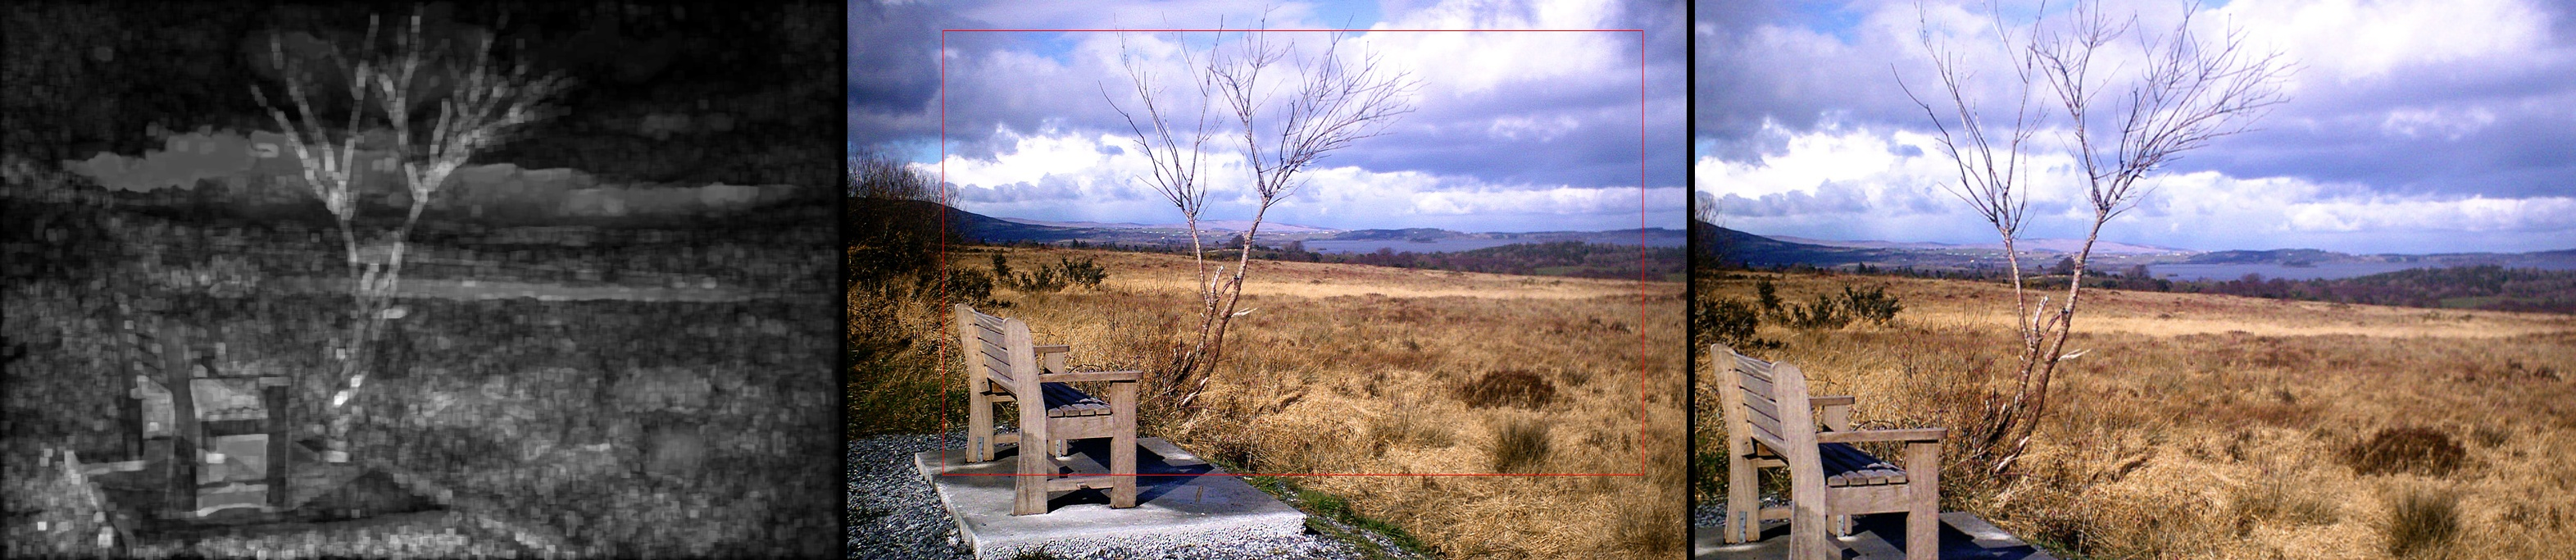
\includegraphics[width=11.5cm]{../figures/good_crops/109123697_Large.jpg}
\vskip2mm
\centering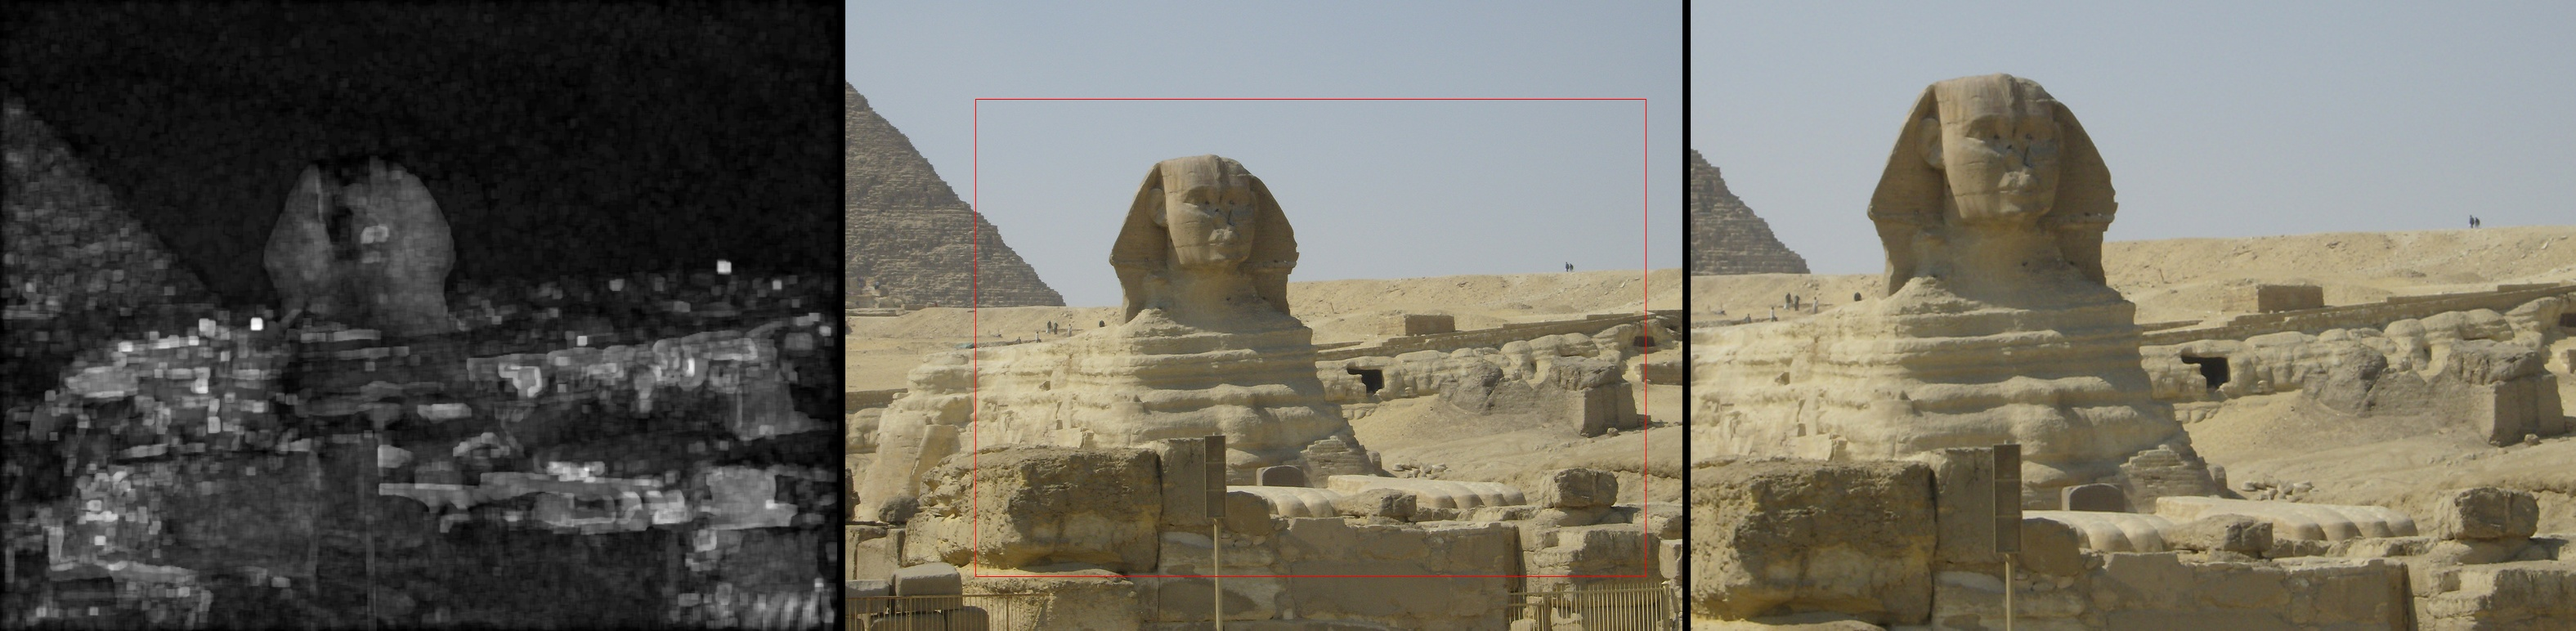
\includegraphics[width=11.5cm]{../figures/good_crops/1158647496_Large.jpg}
\end{figure}
\clearpage

\ETHminimal
\textbf{Results: Cropping (Good)}
\begin{figure}[h!]
\centering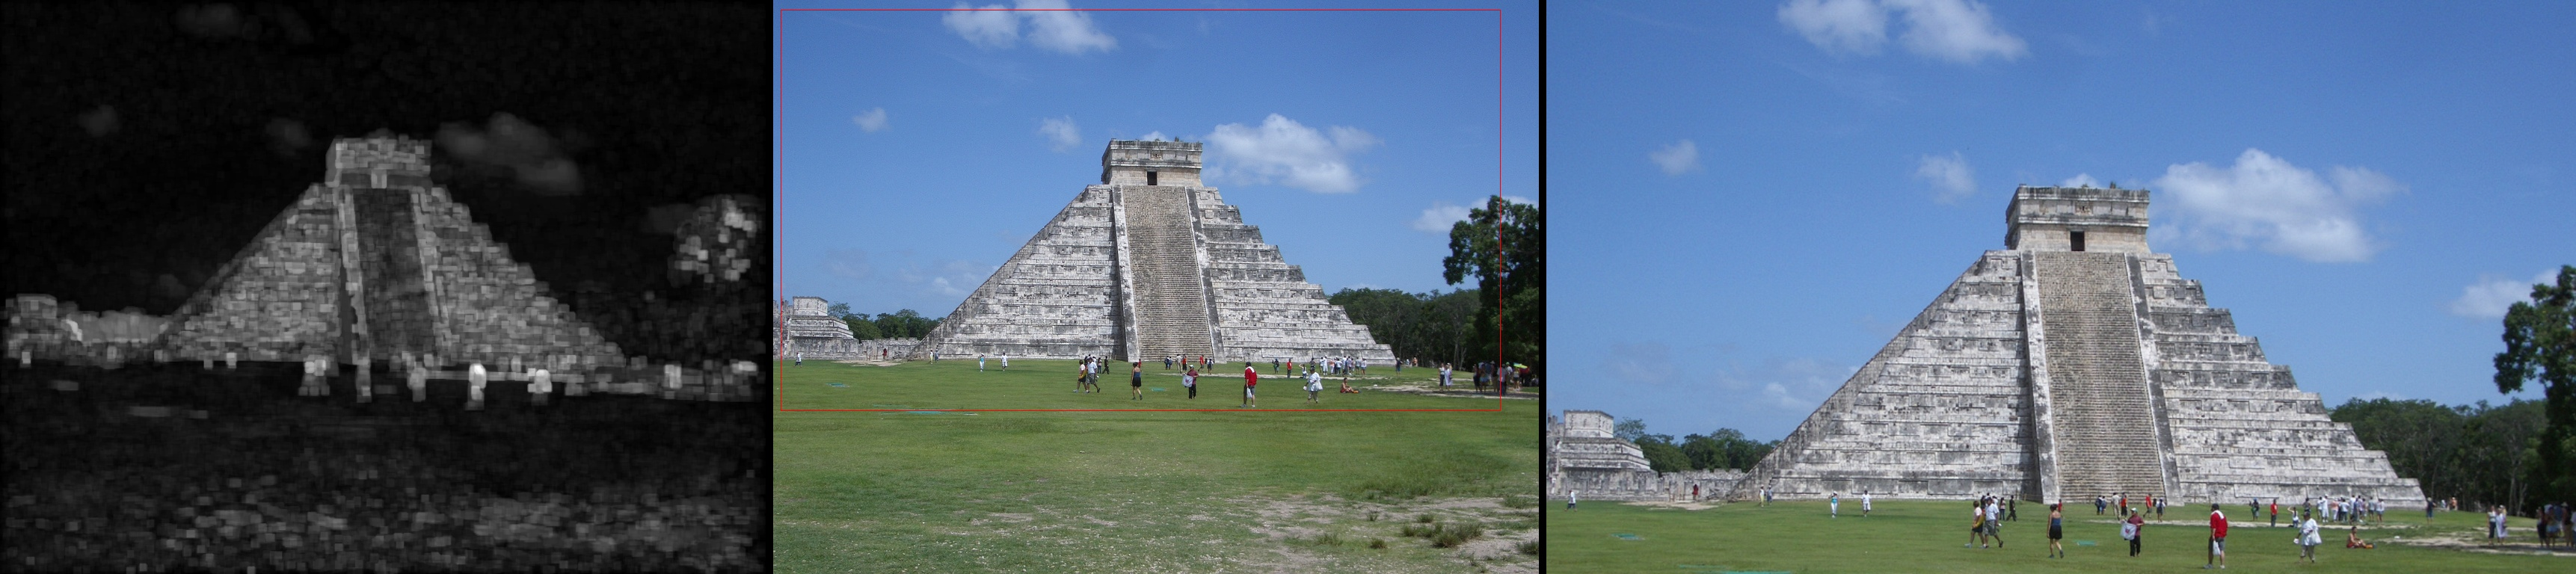
\includegraphics[width=11.5cm]{../figures/good_crops/236441280_Large.jpg}
\vskip2mm
\centering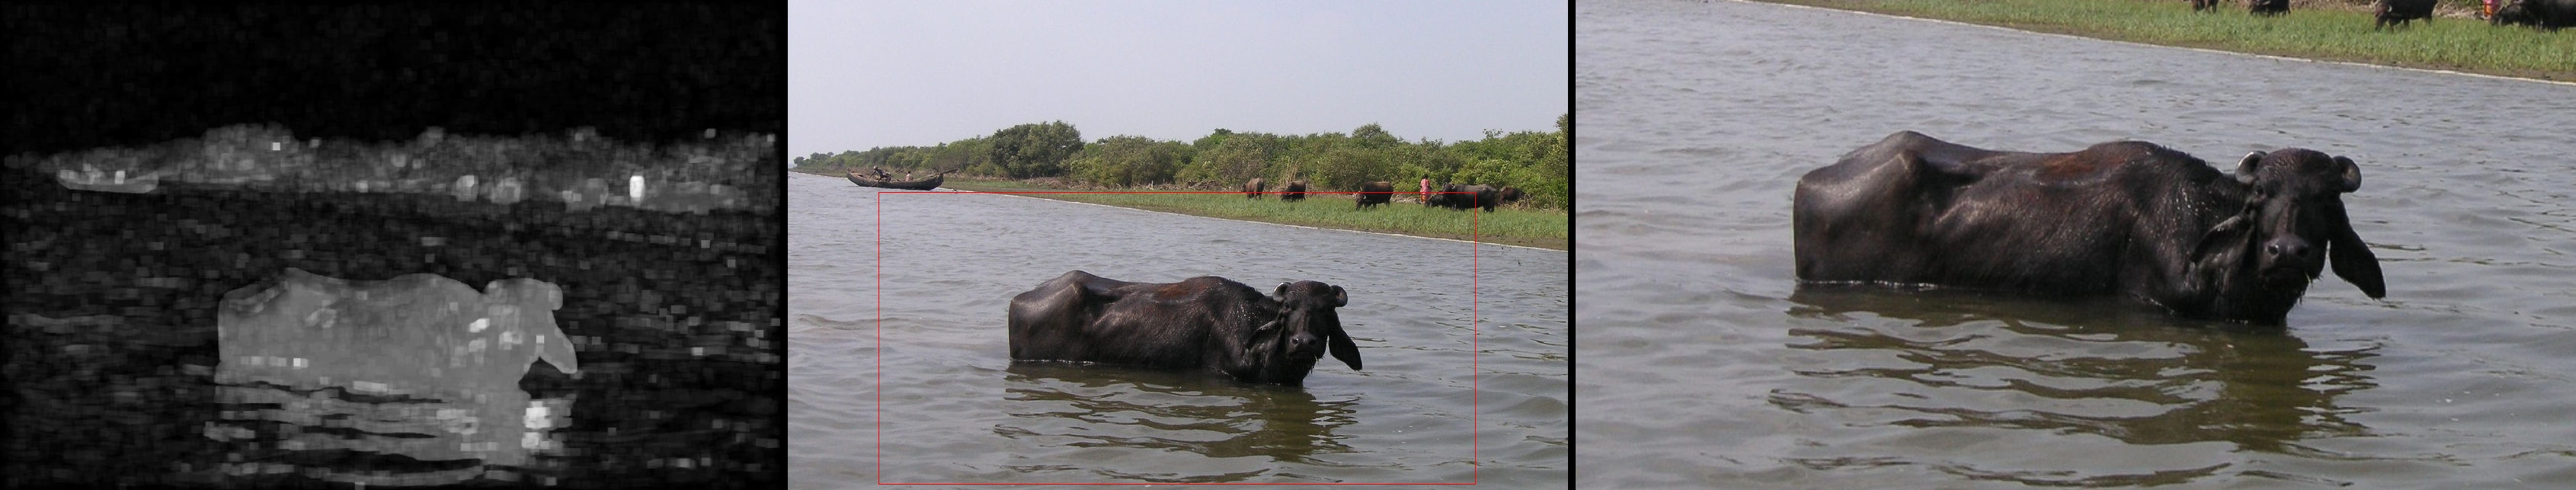
\includegraphics[width=11.5cm]{../figures/good_crops/371485783_Large.jpg}
\end{figure}
\clearpage

\ETHminimal
\textbf{Results: Cropping (Good)}
\begin{figure}[h!]
\centering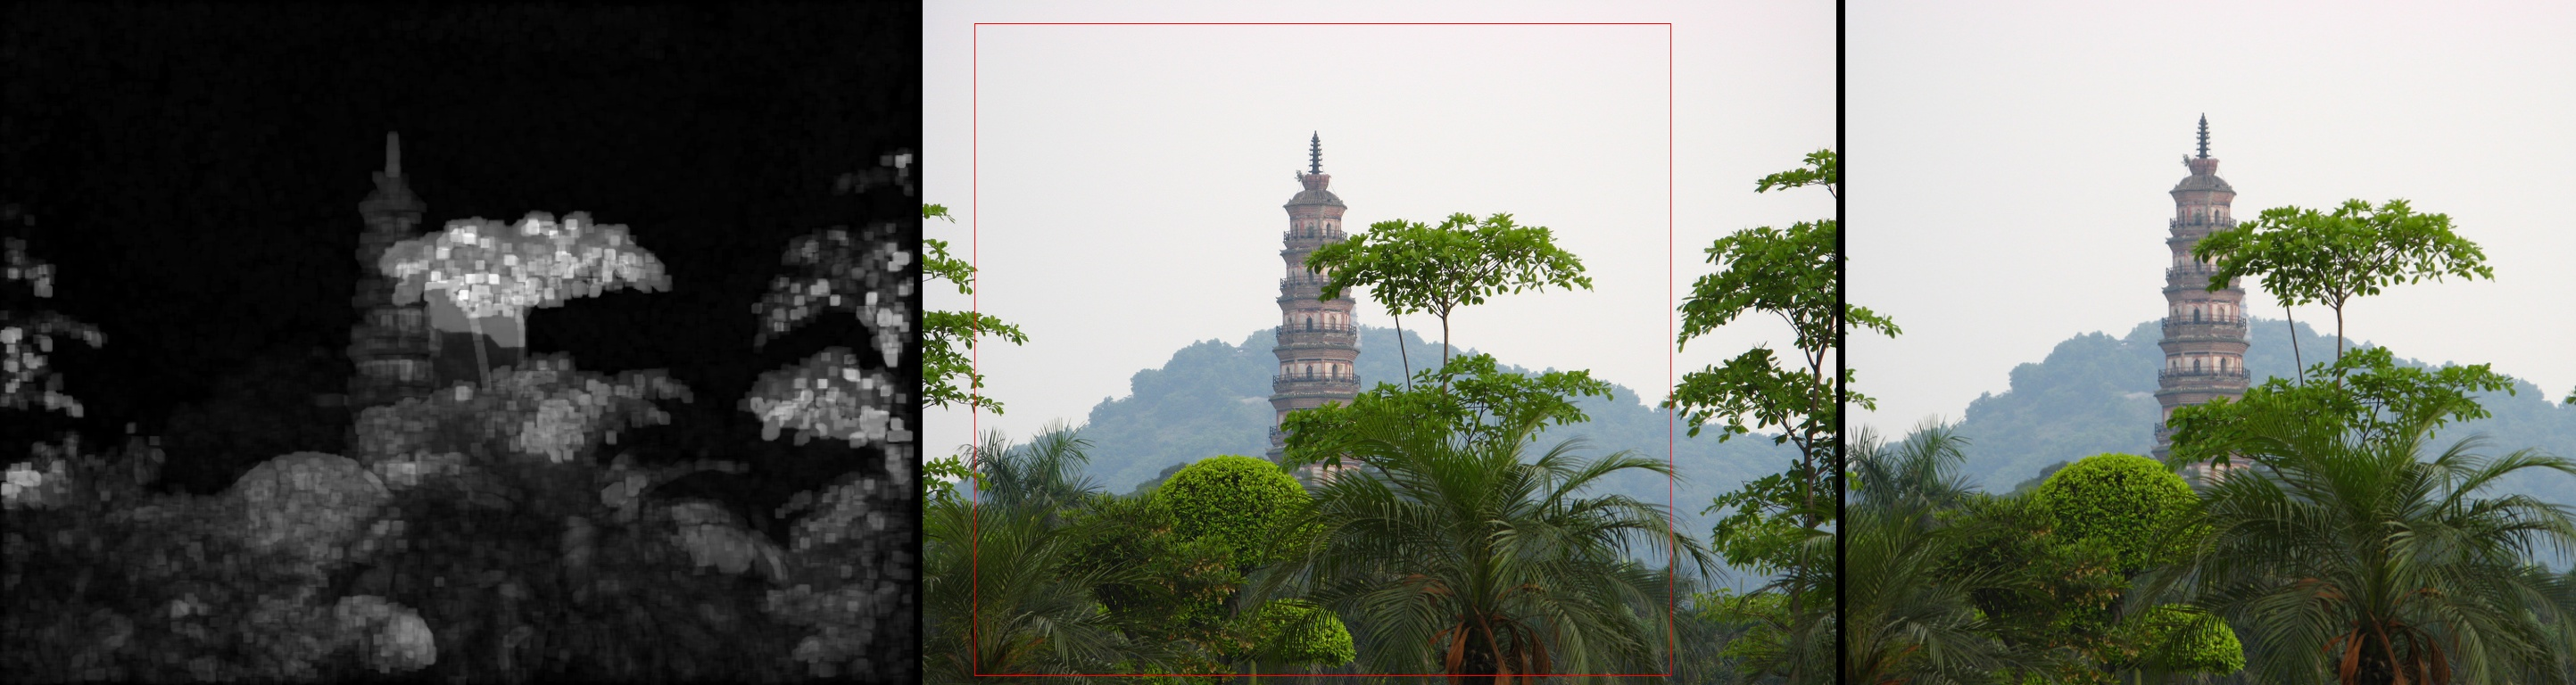
\includegraphics[width=11.5cm]{../figures/good_crops/504325680_Large.jpg}
\vskip2mm
\centering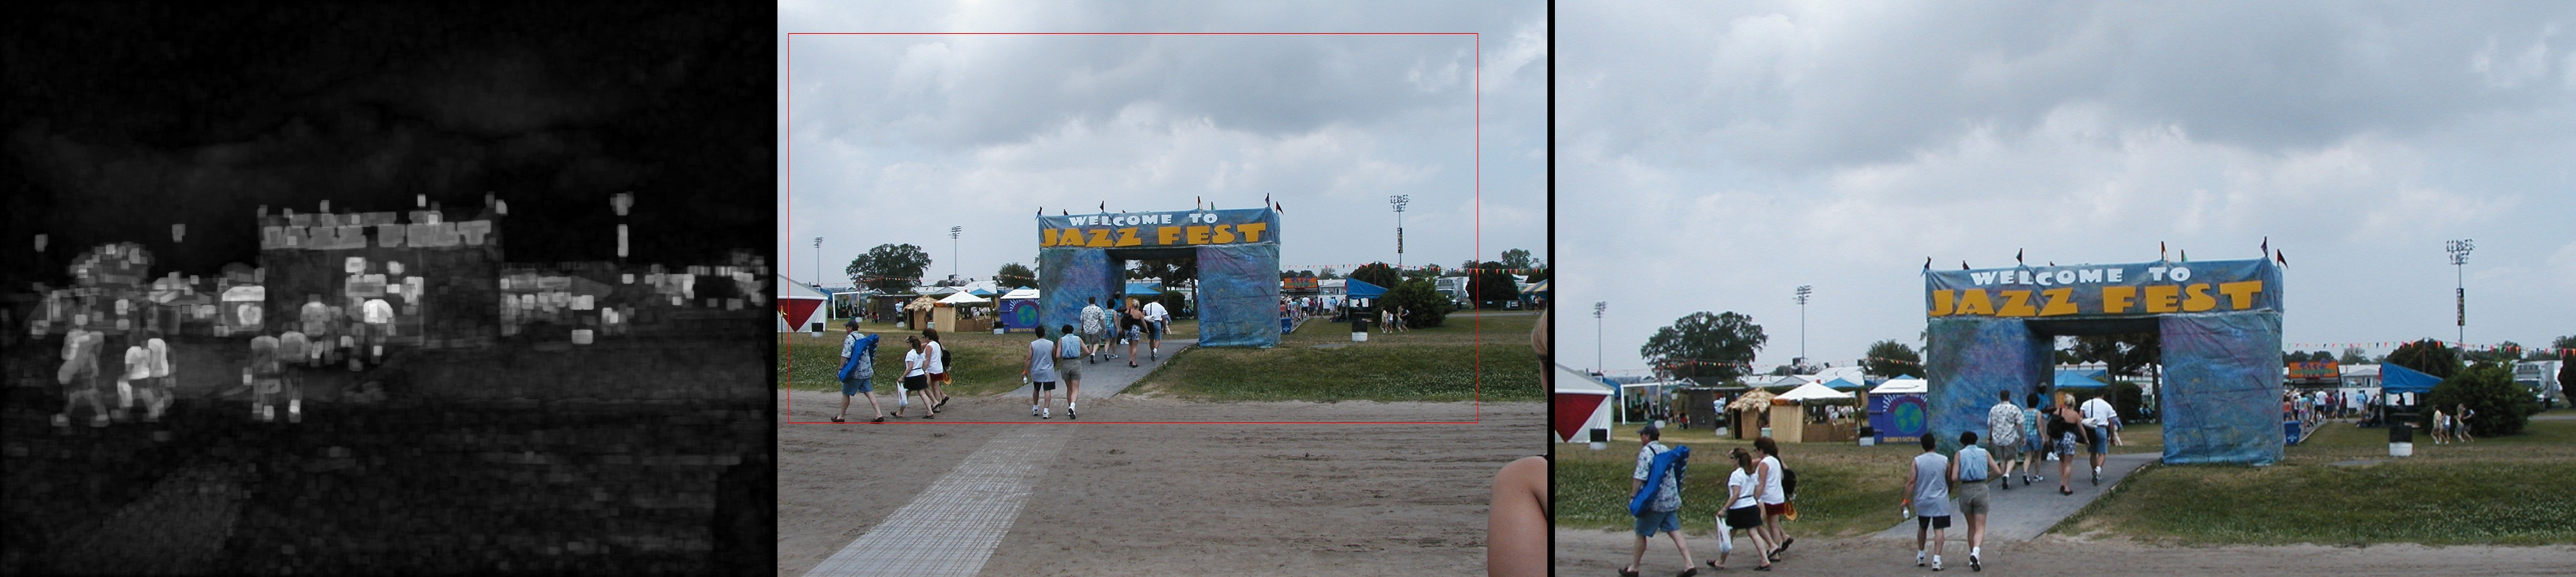
\includegraphics[width=11.5cm]{../figures/good_crops/52968615_Large.jpg}
\end{figure}
\clearpage


\ETHminimal
\textbf{Results: Cropping (Bad)}
\begin{figure}[h!]
\centering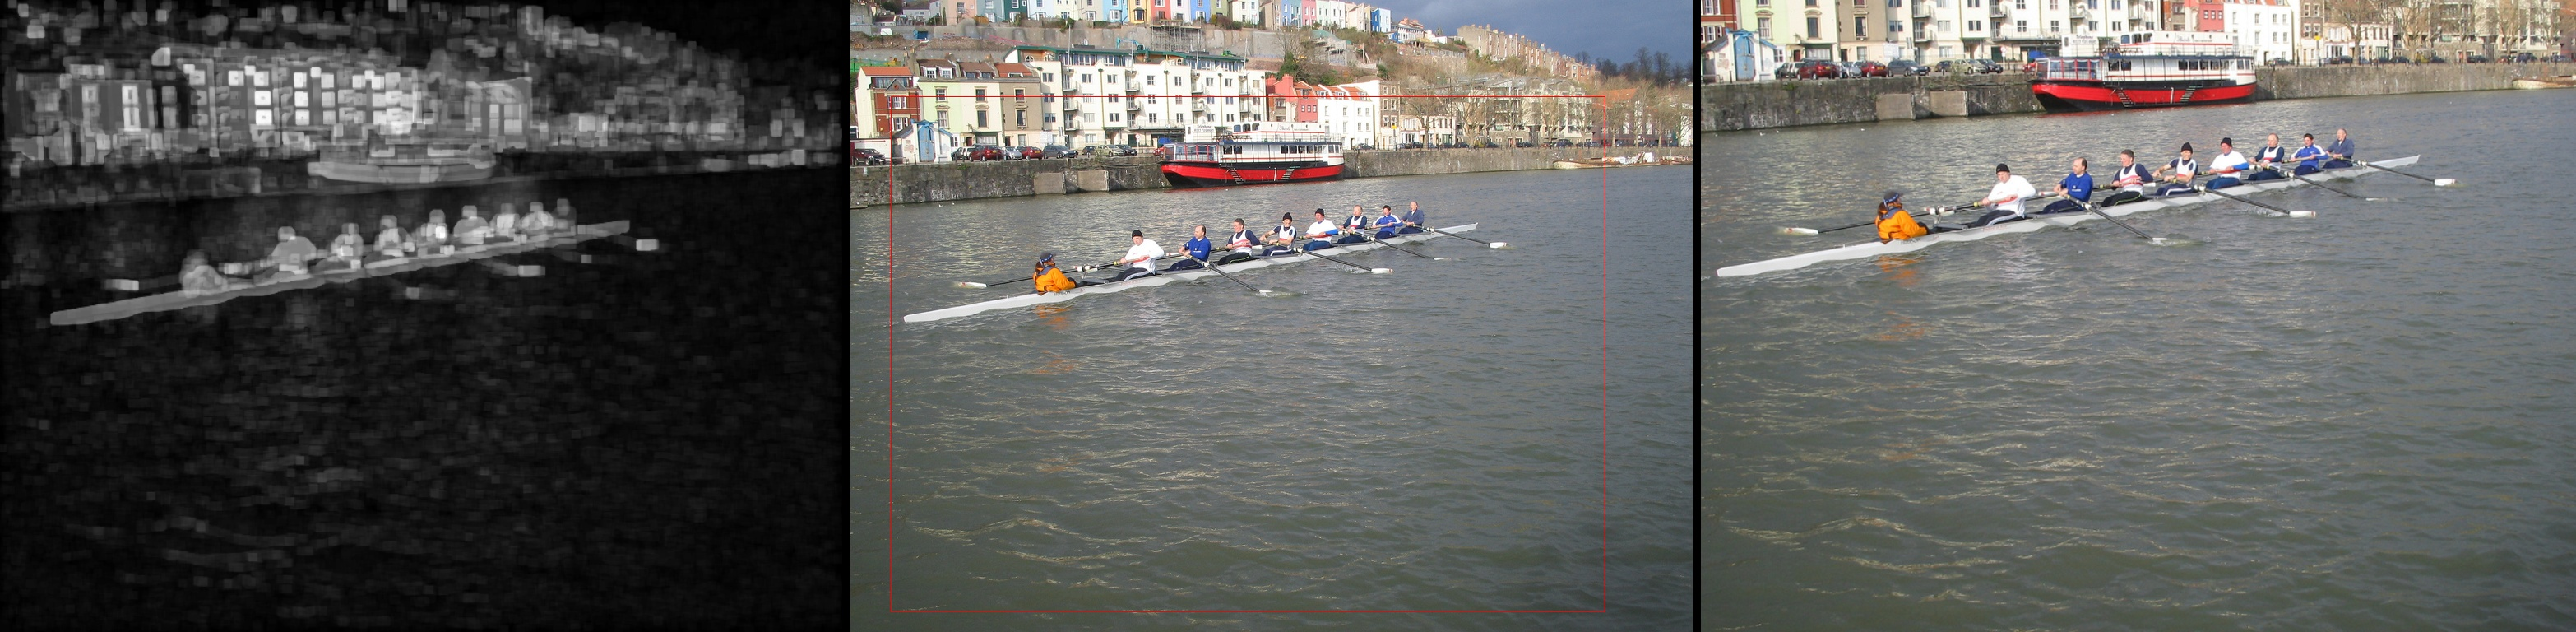
\includegraphics[width=11.5cm]{../figures/bad_crops/104726217_Large.jpg}
\vskip2mm
\centering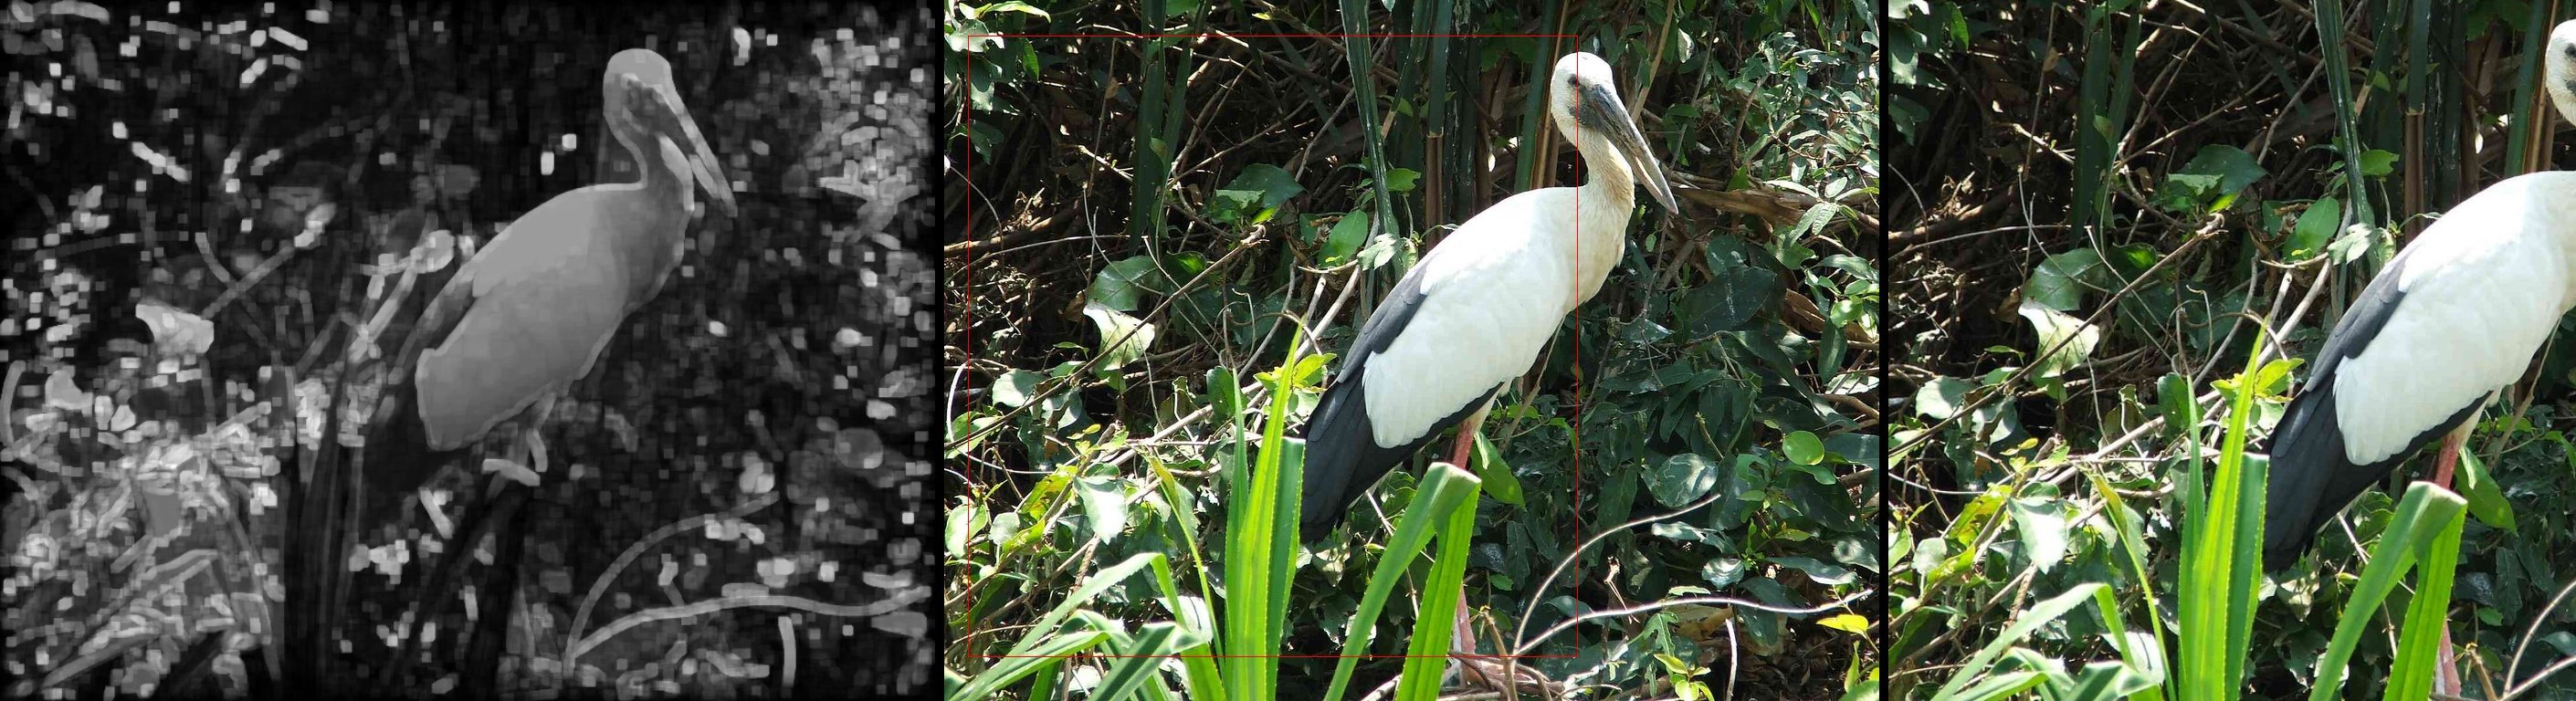
\includegraphics[width=11.5cm]{../figures/bad_crops/118697470_Large.jpg}
\end{figure}
\clearpage

\ETHminimal
\textbf{Results: Cropping (Bad)}
\begin{figure}[h!]
\centering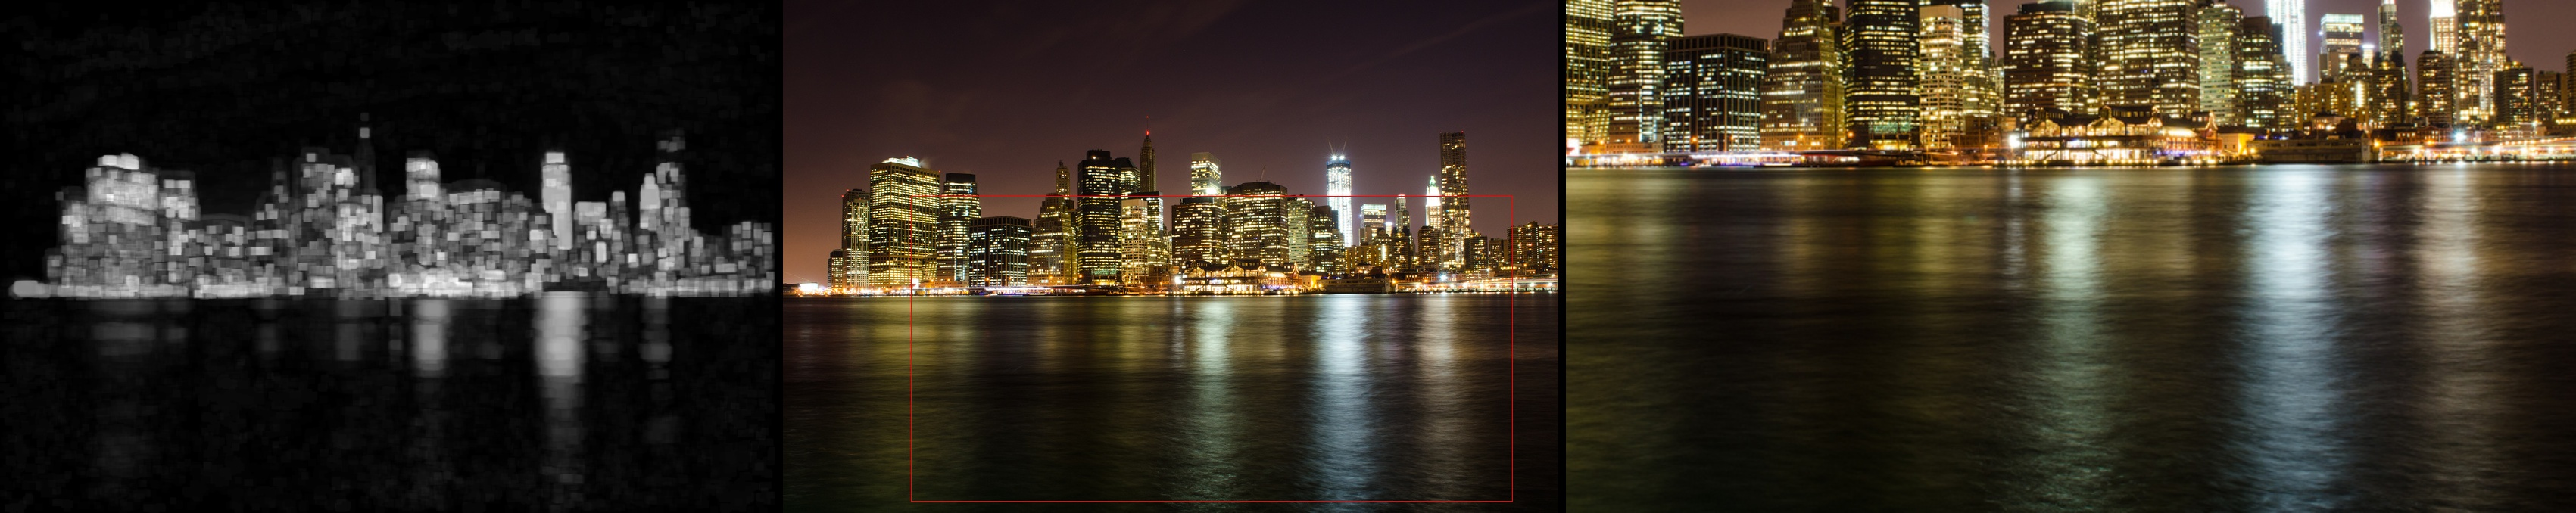
\includegraphics[width=11.5cm]{../figures/bad_crops/6857081990_Large.jpg}
\vskip4mm
\centering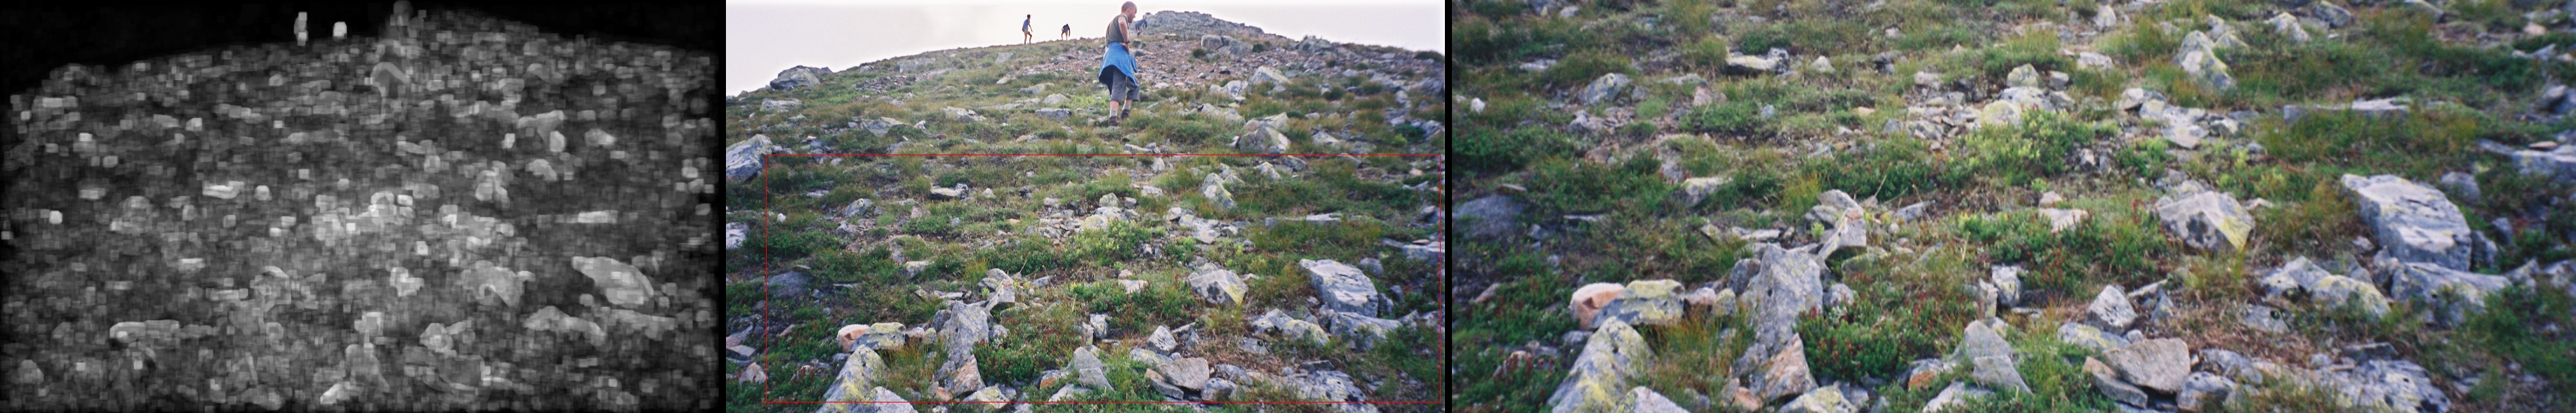
\includegraphics[width=11.5cm]{../figures/bad_crops/119260988_Large.jpg}
\end{figure}
\clearpage

\ETHminimal
\textbf{Analysis: Cropping\\}
\newline
\begin{gather*}
	\mathrm{Overlap}(C_i, H_j) = \frac{C_i \cap H_j}{C_i \cup H_j} \\
	\mathrm{MaxOverlap}(C_i, H) = \max_j\mathrm{Overlap}(C_i, H_j)
\end{gather*}
\begin{itemize}
	\item $C_i$ is the $i$-th crop candidate, and
	\item $H_j$ is the $j$-th human crop. There are $10$ human crops per image.
	\item $\mathrm{MaxOverlap}$ is calculated for $i\in\{1, 2, 3, 4, 5\}$.
	\item $C_0$ is the highest scoring crop.
\end{itemize}
\clearpage

\ETHminimal
\textbf{Analysis: Cropping}
\begin{figure}[h!]
\centering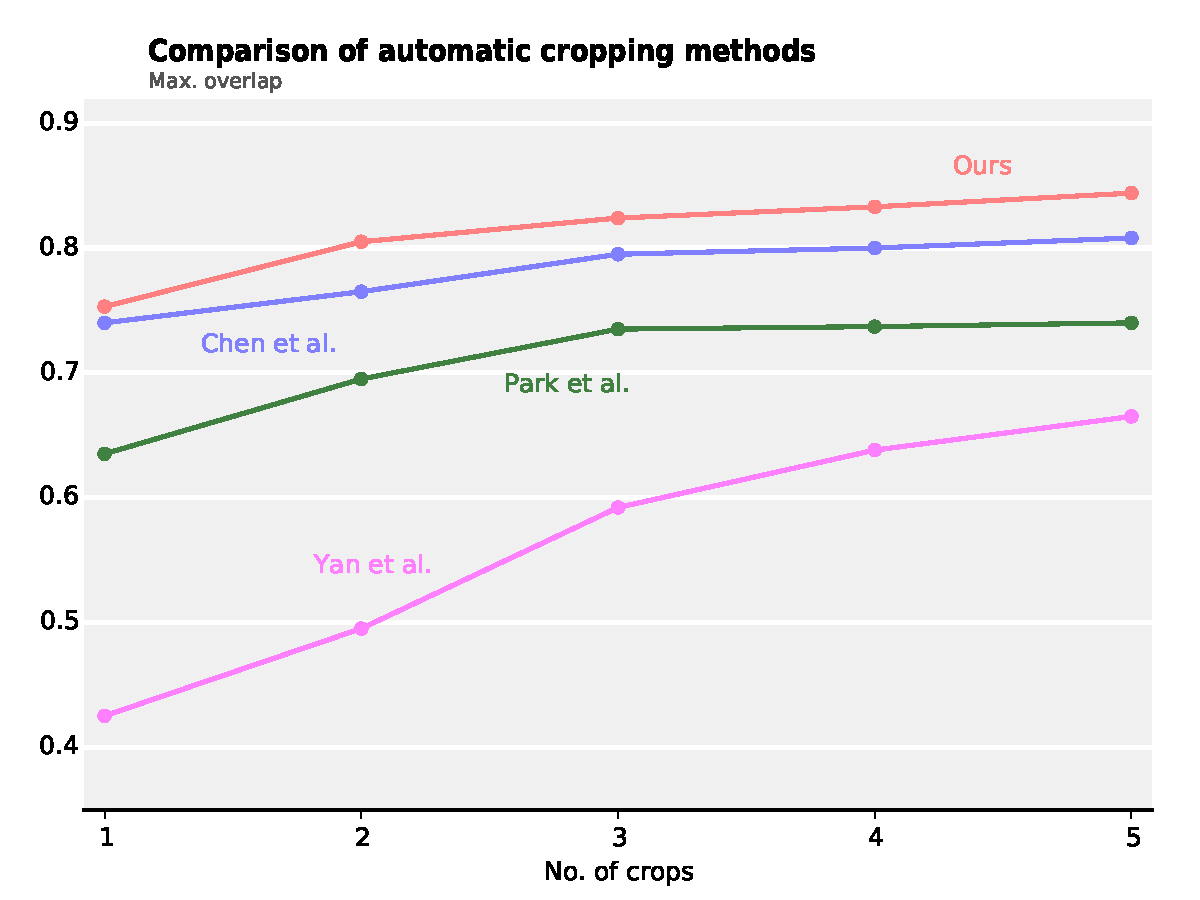
\includegraphics[width=9.3cm]{../figures/comparison.pdf}
\end{figure}
\clearpage

\ETHminimal
\textbf{Summary\\}
\begin{itemize}
	\item
\end{itemize}
\clearpage

\ETHminimal
\textbf{Further Work\\}
\begin{itemize}
	\item
\end{itemize}
\clearpage


%% =========== begin of the standard page ============
%\ETHminimal%
%% ==== start here with the text
%%\tableofcontents
%\textbf{New colors and their names\\}
%Here we show the different colors you can use. From left to right, this are the colors ETH1, ETH2, \ldots , ETH9.
%\newcommand{\quadrat}{(0,0mm)--(0mm,5mm)--(5mm,5mm)--(5mm,0mm)--(0mm,0mm);}
%\begin{center}
%	\hspace{-8mm}
%	\begin{tikzpicture}[overlay]
%		{\draw[ETHa,fill=ETHa] \quadrat}\label{ETH1}
%	\end{tikzpicture}
%	\hspace{10mm}
%	\begin{tikzpicture}[overlay]
%		{\draw[ETHb,fill=ETHb]\quadrat}\label{ETH2}
%	\end{tikzpicture}
%	\hspace{10mm}
%	\begin{tikzpicture}[overlay]
%		{\draw[ETHc,fill=ETHc]\quadrat}\label{ETH3}
%	\end{tikzpicture}
%	\hspace{10mm}
%	\begin{tikzpicture}[overlay]
%		{\draw[ETHd,fill=ETHd] \quadrat}\label{ETH4}
%	\end{tikzpicture}
%	\hspace{10mm}
%	\begin{tikzpicture}[overlay]
%		{\draw[ETHe,fill=ETHe] \quadrat}\label{ETH5}
%	\end{tikzpicture}
%	\hspace{10mm}
%	\begin{tikzpicture}[overlay]
%		{\draw[ETHf,fill=ETHf] \quadrat}\label{ETH6}
%	\end{tikzpicture}
%	\hspace{10mm}
%	\begin{tikzpicture}[overlay]
%		{\draw[ETHg,fill=ETHg] \quadrat}\label{ETH7}
%	\end{tikzpicture}
%	\hspace{10mm}
%	\begin{tikzpicture}[overlay]
%		{\draw[ETHh,fill=ETHh] \quadrat}\label{ETH8}
%	\end{tikzpicture}
%	\hspace{10mm}
%	\begin{tikzpicture}[overlay]
%		{\draw[ETHi,fill=ETHi] \quadrat}\label{ETH9}
%	\end{tikzpicture}
%\end{center}
%\clearpage
%% =========== begin of the standard page ============
%\ETHminimal%
%% ==== start here with the text
%Please use no more then two of them in your presentation. The first two (counted from the left hand side) are reserved for the administration chapter of the ETHZ (first one for external presentation, second for internal), all others you can freely choose.
%
%Please do not forget, fill into your text like in a normal \LaTeX{}-article with the exception that you have to add some additional newline-commands into.
%
%On the following page some example for special commands. And be aware of this minimal ETHZ-page-sample here.
%\clearpage
%% =========== begin of the standard page ============
%\ETHslide%
%% ==== start here with the text
%\textbf{Some mathematical specialities\\}
%\ETHbox{0.8\textwidth}{% define the ETHbox
%  \begin{theorem}[Murphy (1949)]\label{murphy}
%    Anything that can go wrong, will go wrong.
%  \end{theorem}
%}
%
%\begin{proof}
%  A special case of Theorem \ref{murphy} is proven in %\citet{matthews1995}.
%\end{proof}
%
%\ETHitem \quad ETHitem\\
%
%\begin{remark}
%Do not confuse \ETHblue{Murphy's Law} with \ETHbrown{Muphry's Law} by \textit{John Bangsund} which says that ``if you write anything criticizing editing or proofreading, there will be a fault of some kind in what you have written.''
%\end{remark}
%\clearpage
%% =========== begin of inverseseite (inverse page) ============
%\ETHinverseseite\textcolor{white}{\large\textbf{Conclusion}}\\~\newline\hspace{6mm}\normalsize%
%%%
%% ==== start here with the text on the titlepage
%%%
%\textcolor{white}{This is the example inverse page. And we showed, that you can use \LaTeX{} to prepare a presentation very easily.}
%\clearpage
\end{document}
